\subsubsection{2.1. Mạng noron tích chập (CNN)}
\indent\indent Mạng noron tích chập (CNN) \cite{Goodfellow-et-al-2016} là kiến trúc mạng noron sâu nền tảng trong lĩnh vực thị giác máy tính, được thiết kế chuyên biệt để xử lý dữ liệu có cấu trúc dạng lưới như hình ảnh. Khác với mạng noron truyền thống (MLP) với các kết nối dày đặc, có thể dẫn đến bùng nổ tham số, CNN áp dụng cơ chế \textit{tích chập} (convolution) thường được dùng trong xử lý ảnh. Điều này cho phép mạng tự động trích xuất các đặc trưng phân cấp từ thấp (cạnh, góc) đến cao (vật thể hoàn chỉnh) một cách hiệu quả mà vẫn tối ưu được tài nguyên tính toán, nhờ số lượng tham số nhỏ.\vspace{0.3cm}

\begin{figure}[H]
    \centering
    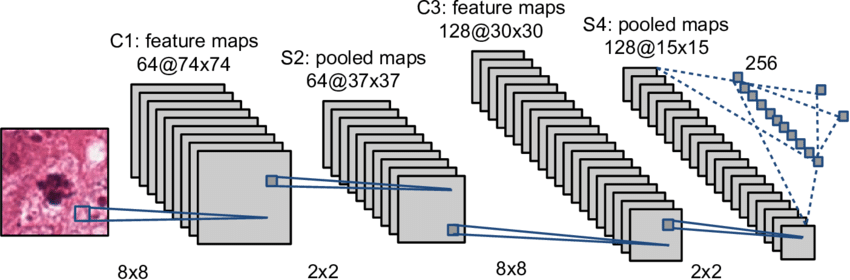
\includegraphics[width=0.8\linewidth]{images/part-02/chap-01/CNN.png}
    \vspace{0.5cm}
    \caption{Minh hoạ kiến trúc cơ bản của CNN}
    \label{fig:CNN}
\end{figure}

Một kiến trúc CNN tiêu chuẩn thường được cấu thành từ sự kết hợp của các tầng sau:\vspace{-0.1cm}
\begin{itemize}[label={--}, itemsep=1pt]
    \item \textbf{Convolutional Layer (Tầng tích chập):} Thành phần nòng cốt thực hiện quét các bộ lọc (filter/kernels) qua đầu vào để tạo ra các bản đồ đặc trưng (feature maps), giúp nhận diện các mẫu cục bộ.
    \item \textbf{Activation Function (Hàm kích hoạt):} Áp dụng các hàm phi tuyến (như ReLU) để giúp mạng có khả năng học được các biểu diễn dữ liệu phức tạp.
    \item \textbf{Pooling Layer (Tầng gộp):} Có công dụng giảm chiều dữ liệu, thường dùng Max Pooling hoặc Average Pooling, giúp giảm chi phí tính toán và tạo ra tính bất biến với các dịch chuyển nhỏ trong ảnh.
    \item \textbf{Fully Connected Layer (Tầng kết nối đầy đủ):} Tổng hợp các đặc trưng đã trích xuất để thực hiện nhiệm vụ cuối cùng như phân lớp hoặc hồi quy.
\end{itemize}

Trong quá trình phát triển, nhiều kiến trúc CNN tiên tiến đã ra đời và thường được đánh giá dựa trên bộ dữ liệu chuẩn ImageNet, trong số đó, tiêu biểu gồm những kiến trúc sau đây:\vspace{-0.1cm}
\begin{itemize}[label={--}, itemsep=3pt]
    \item \textbf{ResNet (Residual Networks)}: Giải quyết vấn đề triệt tiêu đạo hàm (vanishing gradient) khi huấn luyện mạng rất sâu thông qua cơ chế \textit{skip connections}. Các khối residual blocks học hàm sai biệt $F(x)$ thay vì hàm mục tiêu trực tiếp, cho phép huấn luyện hiệu quả các mạng có độ sâu lên tới hàng trăm tầng \cite{he2015deepresiduallearningimage}.
    
    \item \textbf{DenseNet (Densely Connected Networks)}: Tối ưu hóa luồng thông tin bằng cách kết nối mỗi lớp với tất cả các tầng phía sau theo nguyên tắc feed-forward. Việc tái sử dụng đặc trưng giúp DenseNet đạt hiệu suất cao với số lượng tham số ít hơn so với ResNet truyền thống \cite{huang2018denselyconnectedconvolutionalnetworks}.
    
    \item \textbf{MobileNet}: Là dòng kiến trúc tối ưu cho thiết bị di động. MobileNet sử dụng \textit{Depthwise Separable Convolution} để tách phép tích chập thông thường thành hai bước nhẹ hơn (tích chập theo chiều sâu và tích chập điểm), giảm đáng kể khối lượng tính toán nhưng vẫn giữ được độ chính xác cao \cite{howard2017mobilenetsefficientconvolutionalneural}.

    \item \textbf{ShuffleNet}: Tiếp tục cải thiện hiệu suất trên các thiết bị tài nguyên hạn chế. ShuffleNet giới thiệu hai khái niệm mới là \textit{Pointwise Group Convolution} và \textit{Channel Shuffle}. Kỹ thuật này cho phép thông tin được trao đổi giữa các nhóm kênh (channel groups) khác nhau, giúp mô hình đạt độ chính xác cao hơn MobileNet ở cùng một mức độ phức tạp tính toán.\cite{zhang2017shufflenetextremelyefficientconvolutional}.
    
    \item \textbf{RegNet}: Không tập trung thiết kế một kiến trúc đơn lẻ, RegNet nghiên cứu về network design space. Dựa trên phân tích thống kê, RegNet đề xuất các mô hình có cấu trúc đều đặn, đơn giản nhưng hiệu quả, cân bằng tốt giữa độ sâu, độ rộng và tốc độ thực thi \cite{yokoo2020twostagediscriminativererankinglargescale}.
\end{itemize}